\documentclass[12pt]{article}
\usepackage{xcolor} % for different colour text
\usepackage{tikz} % for figures
\usepackage[utf8]{inputenc}
\usepackage{mathpazo}
\usepackage[section]{placeins}
\usepackage{multirow}
\usepackage[normalem]{ulem}
\usepackage{graphicx}
\usepackage{booktabs}
\usepackage{framed}
\usepackage{float}
\usepackage{lipsum}
\usepackage{mathtools, amsfonts}
\usepackage{siunitx}
\usepackage{amsmath, amssymb} % for bold sybmols
\usepackage{bm} % for bold symbols
\usepackage[acronym]{glossaries} % for abbreviations
\usepackage{enumitem}
\newlist{steps}{enumerate}{1}
\setlist[steps, 1]{label = Step \arabic*:}
%\usepackage{bbold} % for identity matrix sign
\usepackage[colorlinks,allcolors=black,citecolor=blue,urlcolor=blue]{hyperref}
\usepackage[citestyle=apa,style=apa,backend=biber,url=false,uniquename=false, useprefix=true, doi=false]{biblatex}
\AtEveryBibitem{%
  \clearfield{note}%
  \clearfield{urlyear}
  \clearfield{urlmonth}
}
\usepackage{dsfont} % for fancy R
\addbibresource{references.bib} % Imports bibliography file
\DefineBibliographyStrings{english}{%
  circa = {{}ca\adddot},
}

% setting (should go in Style sheet:)
\newcommand{\identity}{\mathbf{I}}
\newcommand{\fundmat}{\vec{\Phi}(t, 0)}
\newcommand{\fundmats}{\vec{\Phi}(t, s)}
\newcommand{\fundmatso}{\vec{\Phi}(s, 0)}
\newcommand{\fundmatsu}{\vec{\Phi}(s, u)}
\newcommand{\fundmattv}{\vec{\Phi}(t, v)}
\newcommand{\xtilde}{\widetilde{\vec{x}}}

% ---------------------------------------------------------------------------
% New commands
\newcommand{\1}{\mathbf{1}}
\newcommand{\boldbeta}{\boldsymbol{\beta}}
\newcommand{\boldut}{\mathbf{u}_i(t)}
\newcommand{\boldepst}{\boldsymbol{\varepsilon}_{ij}(t)}
\newcommand{\Expec}{\mathbb{E}}

\newcommand{\Var}{\operatorname{Var}}
\newcommand{\SE}{\operatorname{SE}}
\newcommand{\Cov}{\operatorname{Cov}}
\newcommand{\diag}{\operatorname{diag}}
\newcommand{\ICC}{\operatorname{ICC}}
\DeclareMathOperator{\vect}{vec}

\newcommand{\add}[1]{\textcolor{blue}{#1}}
\newcommand{\delete}[1]{\textcolor{red}{\sout{#1}}}
\newcommand{\edit}[2]{\textcolor{red}{\sout{#1}} \textcolor{blue}{#2}}

% 
\newcommand{\pkg}[1]{{\normalfont\fontseries{b}\selectfont #1}} \let\proglang=\textsf \let\code=\texttt
% ------- %
\setlength{\textwidth}{16cm}
\setlength{\textheight}{22cm}
\setlength{\hoffset}{-1.4cm}
\topmargin -1cm
% ------- %

\title{GLaRe: A Graphical Tool for Assessing
Losslessness of Latent Feature Representations}
\author{
Emma Zohner,
Edward Gunning,
Giles Hooker and
Jeffrey Morris
}
\date{}

% List accronyms we will use for consistency
% \makeglossaries

% \newacronym{fclm}{FCLM}{functional concurrent linear model}

% \newacronym{fda}{FDA}{Functional Data Analysis}

% \newacronym{pda}{PDA}{Principal Differential Analysis}

% \newacronym{ols}{OLS}{ordinary least squares}

% \newacronym{shm}{SHM}{simple harmonic motion}

% \newacronym{scb}{SCB}{Simultaneous confidence band}


\begin{document}

\maketitle



\begin{abstract}
% Advances in modern data collection technologies have led to a proliferation of complex, structured and high-dimensional objects, such as images and curves, for data analysis.
% A common first step in statistical modelling is to learn a latent feature representation of these objects, i.e., a transformation to a lower-dimensional Euclidean space of latent features.

% {\color{red} add downsides of current work?}

Latent feature representation methods play an important role in the dimension reduction and statistical modeling of high-dimensional complex object data.
However, existing approaches to assess the quality of these methods often rely on single summary statistics, such as average or total loss, which can mask variation across individual observations.
We argue that controlling average performance is insufficient to guarantee that statistical analysis in the latent space reflects the data-generating process and instead advocate for controlling the worst-case generalization error, or a larger quantile of the generalization error distribution.
Our framework, CoLLaRe (Compact (near-)Lossless Latent Representations), introduces a systematic way to balance compactness of the representation with preservation of information when assessing and selecting among latent feature representation methods. 
To facilitate its application, we have developed GLaRe\footnote{\url{https://github.com/edwardgunning/GLaRe}}, an open-source \proglang{R} package that implements the framework and provides graphical summaries of the full generalization error distribution.
We demonstrate the utility of CoLLaRe through three case studies on high-dimensional datasets from diverse fields of application.
We apply the CoLLaRe framework to select among principal components, wavelets and autoencoder representations for each dataset.
The case studies reveal that the optimal latent feature representation varies depending on dataset characteristics, emphasizing the importance of a coherent evaluation framework.


% We present GLaRe, a software tool to assess the performance of latent feature representation methods \jsm{for high-dimensional complex object data}.
% GLaRe computes and summarizes the full cross-validated distribution of information losses for a {\jsm linear or nonlinear} latent feature representation method\jsm{,} can be used to select among different methods to represent a dataset \jsm{and choose a latent feature dimension to accomplish a desired level of near-losslessness}

\end{abstract}

\clearpage

\tableofcontents

\clearpage
\section{Introduction}

Advancements in computer storage capabilities and computational speed have made high-dimensional complex data ubiquitous in all areas of science. A common approach for effciently analyzing and modeling these complex objects is to find a low-rank representation that retains the salient characteristics of the data without a significant information loss.
\add{
We use the term \emph{latent feature representation method} to refer to statistical and machine learning approaches that achieve this dimension reduction through a (linear or non-linear) transformation of the data to a lower-dimensional space of features.}
\add{Examples of feature representation methods include} principal components analysis (PCA), independent component analysis (ICA), canonical correlation analysis (CCA), isomaps, non-negative matrix factorization (NMF), linear discriminant analysis (LDA), sparse coding, wavelet transform, t-distributed stochastic neighbor embedding (t-SNE), uniform manifold approximation and projection (UMAP) and auto-encoders. 
These methods aim to retain the dominant characteristics of data in a lower dimensional structure, thereby reducing its dimension. 
In practice, one computes the lower dimensional representation, then applies standard statistical and machine learning tools to the new features. 
For example, these new features can be used as predictors in multivariable regression \add{or} classification, in clustering, or \add{as the} response \add{vector} in multivariate regression \add{models}.

\add{The latent representation space often possess properties for modelling that are more amenable to statistical modelling than the data space, such as
\begin{itemize}
    \item \emph{\underline{Sparsity/ Compression}}: The latent representation space can be of dimension much smaller than the observed data. A compact representation can reduce storage requirements and computational effort in downstream analysis. For example, dimension reduction is used extensively in image compression to minimize the size of graphics files while keeping the quality of the image to an acceptable level \parencite{marcellin_overview_2000}.
    \item \emph{\underline{Regularisation}}: Models and algorithms applied to the latent features often benefit in performance from a reduction of noise and collinearity in high-dimensional data. For example, dimension reduction has been shown to improve results in clustering \parencite{niu_dimensionality_2011}, classifcation \parencite{wang_role_2014} and regression \parencite{cook_fisher_2007}.
    \item \emph{\underline{Visualisation and Interpretation}}: Lower-dimensional latent representations often facilitate intuitive and interpretable visualisations of high dimensional data structures, e.g., for curve or single-cell data objects \parencite{jones_displaying_1992, maaten_visualizing_2008, hyndman_rainbow_2010, becht_dimensionality_2019}.
\end{itemize}}

Since these lower rank representations of the data are used in downstream analyses, any information that is lost in the latent feature representation step is lost in all subsequent analyses. Therefore, it is important to quantify how much information is retained in the representation. 
In fact, the key question in latent feature representation techniques is how well new features capture the information in the data.
Assessing information loss on the same data used to learn the representation will typically result in estimates that overly optimistic.
\emph{Generalization error}, \add{which can be defined as a latent feature representation method's error in reconstructing unseen data, can be used to answer this question and accurately quantify information loss in latent feature representation. 
There is a rich literature on analytical and empirical generalization error for dimension reduction, with a particular focus on cross-validation approaches for PCA \parencite[see, e.g.,][]{becht_dimensionality_2019, wold_cross-validatory_1978, eastment_cross-validatory_1982,krzanowski_cross-validation_1987, minka_automatic_2000, rajan_bayesian_1994, camacho_cross-validation_2014, diana_cross-validation_2002, hubert_fast_2007, josse_selecting_2012, saccenti_use_2015}}.


% [6], [7], [8], [9], [10], [11], [12], [13], [14], [15], [16]. 
% Generalization error in the general unsupervised learning context is described in [17].

\add{However, in these papers and more generally in practice, generalization error for latent feature representations is expressed as a single statistic for that summarises the distribution of generalization errors of individual observations e.g., the average \add{or total} error.
Often a single number is not sufficient to characterise the distribution of individual generalization errors, e.g., a respectable average generalization error might mask the fact that a number of observations are being represented poorly. 
To be confident that a given latent feature representation captures the information and structure in an entire dataset, its performance over the full collection of observations needs to be assessed so that features of the generalisation error distribution can be evaluated, e.g., the median, the best case, the worst case and other quantiles.}
% However, to be confident in the degree to which the representation captures the information in the original data, \add{observations} need to be evaluated individually and we want to be confident that the representation keeps the information for a high percentage of \add{observations}.
% To determine whether \add{all (or most of) observations} in the data are well represented, it is necessary to compute performance over the whole distribution so that summaries other than the mean can be made to assess how well the best case, worse case or other quantiles can be evaluated. 

\add{It is also well established that the suitability of a latent feature reprentation depends heavily on the characteristics of the dataset at hand, i.e., there is no preferred ``one size fits all" method.
For example, this has been emphasised in the context of basis function representations for functional data -- curves with different smoothness, regularity and sampling characteristics are suited to different types of basis functions, e.g., wavelets, splines and functional principal components \textcite[Section 3, pp. 325--328]{morris_functional_2015}.
However, most available methods for computing generalization error focus on a single latent feature representation method (e.g., PCA) and do not allow comparison between methods by using similar statistics or summaries.}


In this article, we introduce a Graphical Latent Feature Representation tool (GLaRe) for assessing how well a \add{learned latent feature representation} captures the salient information in a given dataset, allowing the user to select \add{an optimal} representation for the data. The tool is developed in \proglang{R} \parencite{r_core_team_r_2022} and accessible via a \proglang{R} \pkg{Shiny} interface \parencite{chang_shiny_2021}. 
\add{Although there is existing software for dimension reduction which we briefly survey below, the tool that we present is unique in its simultaneous focus on assessing the generalization error for individual observations and facilitating the comparison between multiple latent feature representations.}
\add{\textcite{samudrala_software_2014} developed software for dimension reduction that provides a graphical user interface that outputs an optimal low-dimensional representation, but it does not address generalization of the dimension reduction methods, and it is specifically tailored to chemical crystallography data.
\textcite{zubova_dimensionality_2018} compared the speed and accuracy of dimension reduction and provided visualisations, but generalization error and individual-level performance measures were not provided. 
An \proglang{R} package for a single method, Multifactor Dimensionality Reduction, was developed by \textcite{winham_r_2011}. Visualization of the quality of dimension reduction, as well as point-wise quality measures are discussed by \textcite{mokbel_visualizing_2013} but no software is provided. 
In \textcite{cavallo_visual_2018} a visual interaction framework is presented for dimension reduction where users can directly manipulate and modify data through dimension reduction visualizations. This framework's focus is on interaction via forward and backward projection to improve the use of dimensionality
reduction.}
\add{To summarise, there is a lack of user-friendly software to assess the performance of different latent feature representations at the individual observation level.}

\add{The remainder of this article is structured as follows.
In Section \ref{sec:materials-and-methods}, we present the methodological foundations of latent feature representations and generalisation error, and we introduce three motivating datasets that are used as a case study in this article. 
In Section \ref{sec:software}, we document our novel Graphical Latent Feature Representation (GLaRe) tool.
Section \ref{sec:results} presents the results of our case study, where we use our proposed Graphical Latent Feature Representation (GLaRe) tool to assess the performance of PCA, the Discrete Wavelet Transform (DWT) and and autoencoder representations of our three motivating datasets.
We close with a discussion in Section \ref{sec:discussion}.
}


\section{Methodological Framework (CoLLaRe)}\label{sec:materials-and-methods}

\subsection{Latent Feature Representations}

Suppose that we have $N$ observations of object data, denoted by $X_1 (t), \dots, X_N(t)$, where $t$ indexes a location on a domain $\mathcal{T}$ over which the objects are defined.
For time-varying curves, $\mathcal{T}$ is generally a closed subset of the real line that represents a (normalized) time interval.
However, as exemplified in our three motivating datasets, the domain $\mathcal{T}$ can be multi-dimensional to represent locations in an image or surface, and it can also be non-Euclidean ({see Glaucoma data/ \textcite{lee_bayesian_2019}}).
We assume that each observation is measured on a common\footnote{In practice, the measurement grids of individual observations need not be identical if they are all sufficiently fine such that interpolation onto a common, fine grid is feasible.}, ordered grid of $T$ points in $\mathcal{T}$, denoted by $\mathbf{t} = \left(t_1, \dots, t_T\right)^\top$, and we let $X_i(\mathbf{t}) = \left\{X_i(t_1), \dots, X_i(t_T)\right\}^\top$.
Then, we can represent the observed data in the $N \times T$ data matrix $\mathbf{X}$, which contains the vectors $X_1(\mathbf{t}), \dots, X_N(\mathbf{t})$ in its rows.
We refer to the $T$-dimensional space of features in which the observed data are represented as the \emph{data space}.

We define a \emph{latent feature representation method} as a technique comprising two transformations, known as the \emph{encoding} and \emph{decoding} transforms.
The encoding transform $f_{K}$ transforms an observation from the data space to a new space of latent features, called the \emph{representation space}
$$
f_{K} \left\{X_i(\mathbf{t})\right\} = \left(X_{i1}^*, \dots,  X_{iK}^* \right)^\top,
$$
where the number of features $K$ defines the dimensionality of the representation space and can range between $1$ and some possible maximum $K_{max}$. When $K \ll T$, we say that the latent feature representation is \emph{compact}.
As we expand on in Section \ref{sec:characterising-information-loss}, we typically want the representation space to be as compact as possible.

% space\footnote{If we have have representation of the underlying object $X_i(t)$ that does not involve measurement on a grid, the transformation can be defined on the object itself as $f_{K} \left(X_i(t)\right) = \left(X_{i1}^*, \dots,  X_{iK}^* \right)^\top$.} to a new space of latent features, called the \emph{representation space}, and back-transforms on observation in the latent space of features to the data space, using an inverse transformation.
% Mathematically, we define the latent feature representation of the $i$th observation as



We define the decoding transform as the inverse transformation function $f^{-1}_K$ that maps an observation from the representation space back to the data space as
$$
\widehat{X}_i^{(K)} (\mathbf{t}) = f_{K}^{-1} \left\{ \left(X_{i1}^*, \dots,  X_{iK}^* \right)^\top \right\}.
$$

Linear transformations of the form $f_{K} \left\{X_i(\mathbf{t})\right\} = \mathbf{A} X_i(\mathbf{t})$, for some $K \times T$ transformation matrix $\mathbf{A}$, are often used in practice.
For example, it is common to represent a functional observation $X_i(t)$ as a linear combination of a set of basis functions $\{\phi_k(t)\}_{k=1}^K$, which defines the inverse transformation
$$
\widehat{X}_i^{(K)} (\mathbf{t}) = \sum_{k=1}^K X_{ik}^* \phi_k(\mathbf{t}) = \boldsymbol{\Phi} \left(X_{i1}^*, \dots,  X_{iK}^* \right)^\top,
$$
where $\boldsymbol{\Phi} = \left[\phi_1(\mathbf{t}) | \dots | \phi_K(\mathbf{t}) \right]$ and the latent features $X_{ik}^*$ are basis coefficients. 
When these basis coefficients are computed by ordinary least squares, the linear transformation matrix defining the latent feature representation $f_K$ is of the form $\mathbf{A} = \left( \boldsymbol{\Phi}^\top \boldsymbol{\Phi} \right)^{-1} \boldsymbol{\Phi}^\top$.
When the matrix of basis function evaluations $\boldsymbol{\Phi}$ is orthogonal, $\mathbf{A} = \boldsymbol{\Phi}^\top$, i.e., the transformation $f_K$ is simply right multiplication by this matrix.
However, in general, there is no need for the transformation $f_K$ to be orthogonal or even linear, and non-linear transformations may be preferred for certain types of data.

Although statistical modeling is performed in the representation space due to its attractive properties, we often want to transform modeling results back to the data space for inference, interpretation and visualization. 
As such, the accuracy and interpretation of an analysis depends on the degree of information that is preserved when moving back and forth between the data and representation spaces for a given latent feature representation.
In what follows, we characterize the degree of information loss of a latent feature representation on a full dataset.


\subsection{Characterizing the Full Distribution of Information Loss}\label{sec:characterising-information-loss}

We denote the degree of information loss of a latent feature representation for each individual observation by 
$$
\text{Loss} \left\{ X_i(\mathbf{t}) \right\} 
= g\left\{ X_i(\mathbf{t}), \widehat{X}_i^{(K)}(\mathbf{t}) \right\},
$$
where the $g$ is a symmetric, non-negative function that measures dissimilarity between $X_i(\mathbf{t})$ and $\widehat{X}_i^{(K)}(\mathbf{t})$, and satisfies $g\left\{ X_i(\mathbf{t}), \widehat{X}_i^{(K)}(\mathbf{t}) \right\}=0$ when $X_i(\mathbf{t})=\widehat{X}_i^{(K)}(\mathbf{t})$.
For example, $g$ could be the Euclidean distance between $X_i(\mathbf{t})$ and $\widehat{X}_i^{(K)}(\mathbf{t})$ \parencite{morris_comparison_2017}, or the complement of a similarity measure such as a squared correlation or concordance index \parencite{yang_quantile_2020}.
We say that the transformation $f_K$ is \emph{lossless} for the $i$th observation if
$$
\text{Loss} \left[ f_K\{X_i(\mathbf{t})\} \right] = 0,
$$
and lossless for the full dataset if
$$
\text{Loss} \left[ f_K\{X_i(\mathbf{t})\} \right] = 0 \quad \forall \quad  i = 1, \dots, N.
$$
That is, we only refer to a latent feature representation as (near) lossless for a given dataset if the representation is (near) lossless for every individual observation in that dataset.
More generally, we can allow some tolerance of information loss and say that
the transformation $f_K$ is \emph{near-lossless} for the $i$th observation if
$$
\text{Loss} \left[ f_K\{X_i(\mathbf{t})\} \right] < \epsilon,
$$
for a chosen tolerance level $\epsilon$. 
Similarly, we say that the transformation $f_K$ is near-lossless for the full dataset only if each individual observation achieves this tolerance level, that is
$$
\text{Loss} \left[ f_K\{X_i(\mathbf{t})\} \right] < \epsilon \quad \forall \quad  i = 1, \dots, N.
$$
It is important to distinguish this definition from an overall (or total) measure such as the average of individual losses $\frac{1}{N}\sum_{i=1}^N \text{Loss} \left[ f_K\{X_i(\mathbf{t})\} \right]$.

Figure \ref{fig:ind-losses} displays the distribution of individual information losses on a dataset sample dataset of a PCA latent of varying dimensions on the \texttt{phoneme} dataset (a dataset of $1$-dimensional signals, described in more detail in Appendix \ref{sec:additional-data}).
In this case, we are using the complement of the squared correlation as our loss, so a value of $1$ means the representation captures no information and a value of $0$ means that the representation is lossless.
The gray points represent the individual observations' losses, whereas the red squares indicate the average loss.
The figure highlights the information that can be hidden when a single statistic is used to describe the full distribution of losses. For example, at $k = 1$ the average loss is at approximately $0.6$ but there are observations with individual losses at almost $1$, which would indicate that no information is being retained by the transformation.


\begin{figure}
    \centering
    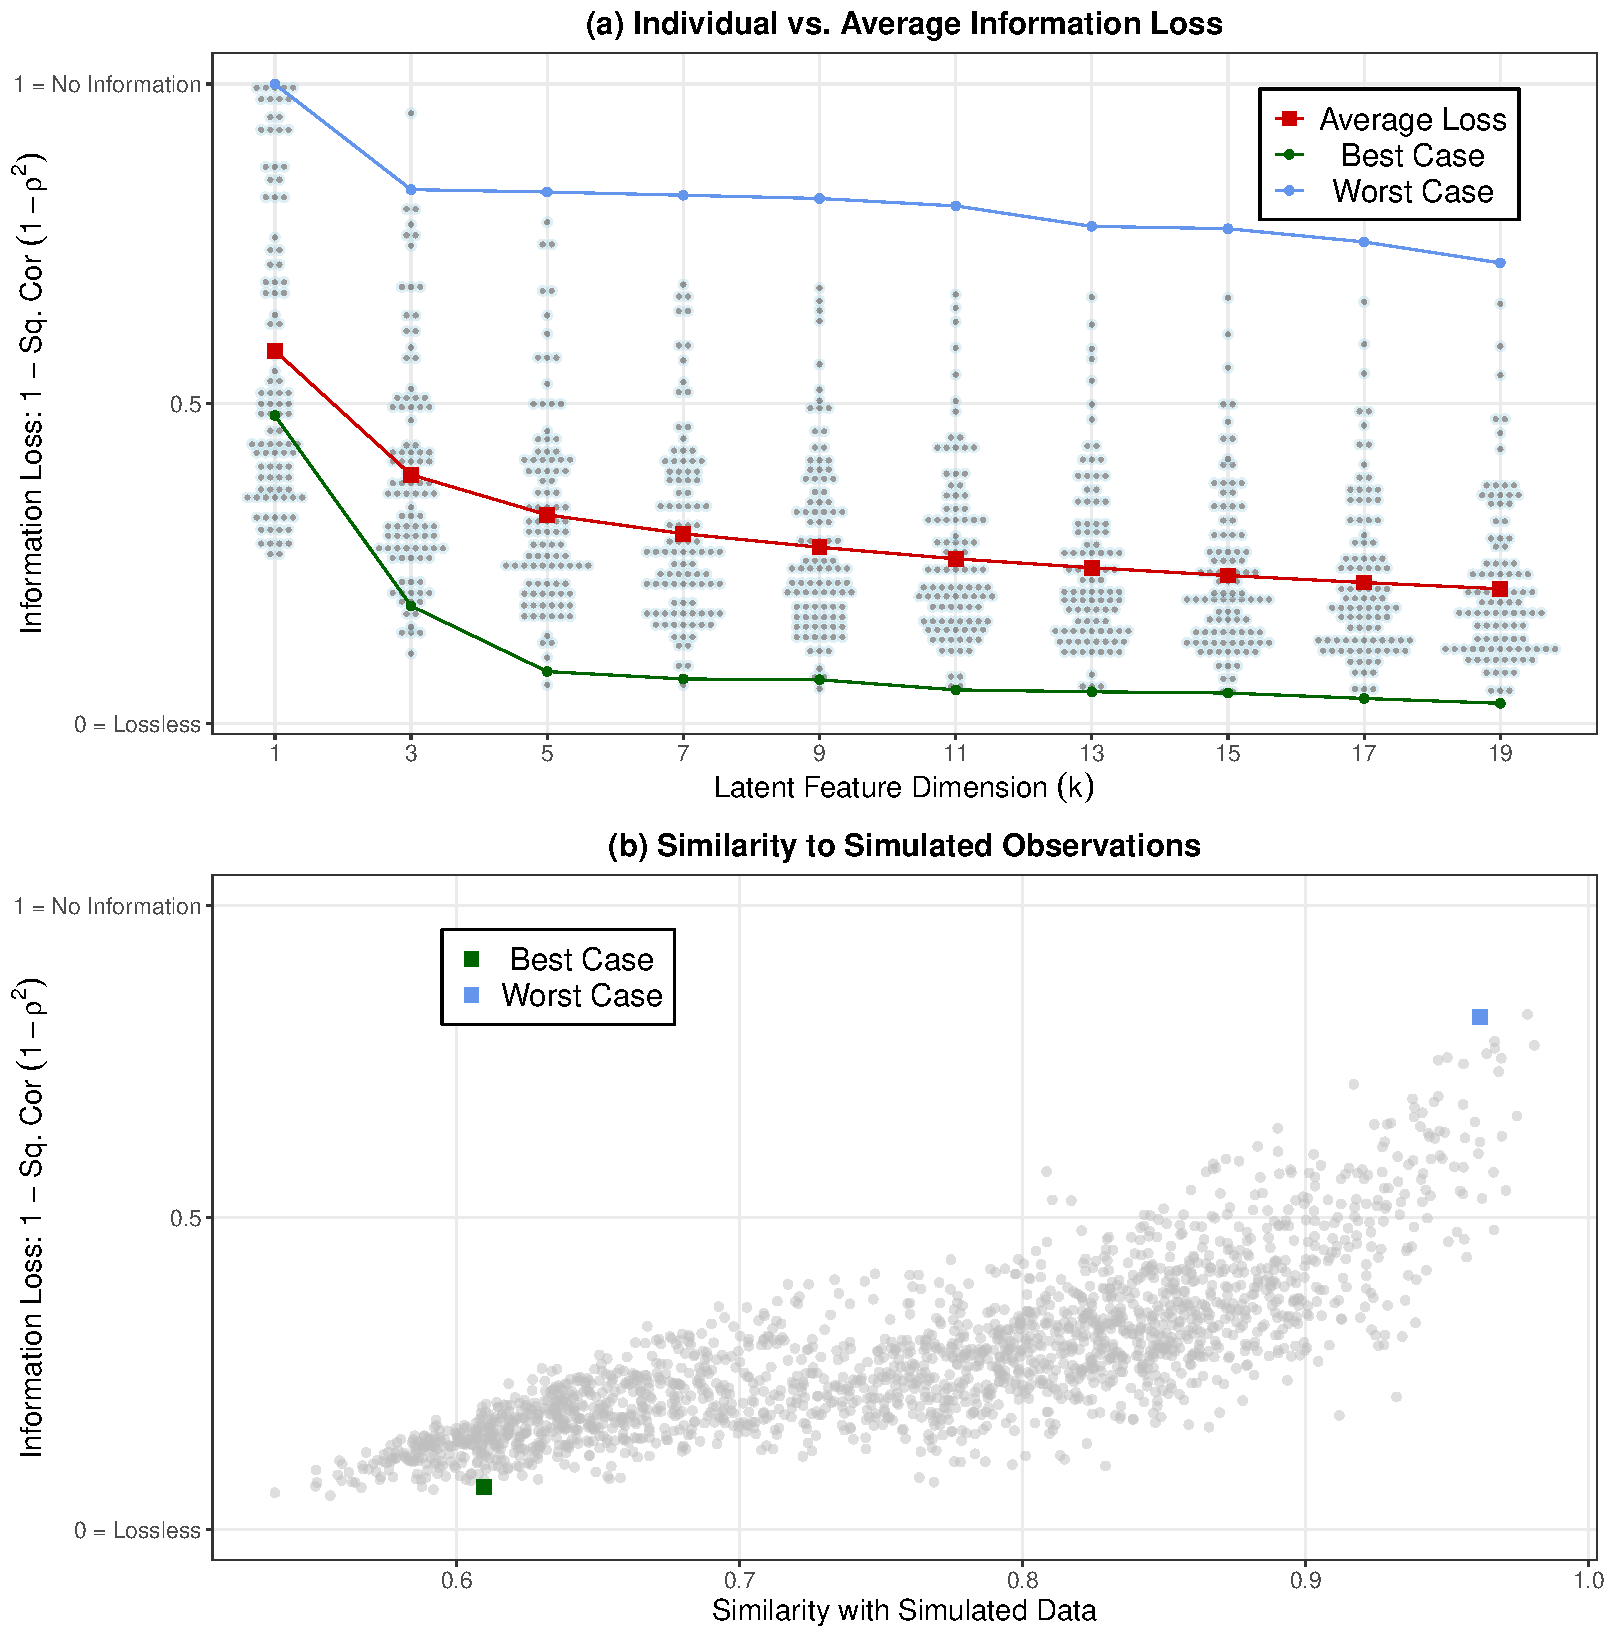
\includegraphics[width=0.75\textwidth]{figures/info-loss-02.pdf}
    \caption{
    \textbf{(a)}: Generalization errors from a PCA representation of the \texttt{phoneme} data (see Appendix \ref{sec:additional-data}). The grey dots represent individual cross-validated reconstruction errors from PCA representations using different numbers of latent features ranging from $1$ to $19$ ($x$ axis).
    The complement of the squared correlation is used as reconstruction loss, so $1$ indicates no information retained by the representation and $0$ indicates a lossless representation ($y$ axis).
    The square red points and solid red line trace the average reconstruction error. The green and blue points / lines trace the performance of the best and worst performing observations (selected at $K=19$), respectively.
    \textbf{(b)}: The same data and representation method in \textbf{(a)} with $K=9$ were used to simulate $N = 100$ observations from the latent space.
    The average dissimilarity (i.e., reconstruction error) between the individual observations and the $N=100$ simulated observations is shown on the $x$-axis and the individual cross-validated reconstruction errors at $K=9$ is shown on the $y$-axis. The scatterplot displays a strong, non-linear positive relationship between the reconstruction errors and dissimilarity to the simulated observations.
    }
    \label{fig:ind-losses}
\end{figure}


Achieving a chosen tolerance level for every observation (i.e., requiring that even the worst case meets the near-losslessness threshold) can sometimes be unrealistic in practice.
Often, a small number of observations (e.g., the one traced by the blue points and line in Figure \ref{fig:ind-losses}) possess idiosyncratic features that cannot be captured by a representation that is otherwise compact and near-lossless for the vast majority of the observations.
In this case, using the worst case is overly stringent and results in a latent feature representation that is higher-dimensional and more complex than required for the vast majority of observations.
Therefore, we generalize the notion of near losslessness for the entire dataset, and require it to be met for \emph{quantiles} or \emph{percentiles} of the distribution of individual generalization errors, in which the worst-case observation is the $100$th percentile. 
As before, $\epsilon$ denotes the tolerance level of information loss that we want to achieve.
We now introduce the \emph{attainment rate}, which we denote by $\alpha$, as the proportion of observations that we want to achieve this tolerance level.
For example, a attainment rate of $\alpha = 0.95$ would indicate that we require $95\%$ of the observations in the dataset to achieve a loss smaller than the tolerance level $\epsilon$.
We refer to a chosen combination of $\epsilon$ and $\alpha$ as the qualifying criterion and we use the term \emph{qualifying dimension (qd)} to denote the smallest latent feature dimension $K$ for which this criterion is satisfied.
When comparing two latent feature representation methods (e.g., PCA and autoencoder), for a fixed $\epsilon$ and $\alpha$, we generally prefer the method with a smaller qualifying dimension as it provides a more compact representation of the dataset.
Finally, we characterize the dimension reduction achieved by a method by its \emph{compression ratio}, which is the ratio of the original data dimension $T$ to the qualifying dimension $qd$, typically rounded to the nearest whole number.

We conclude this section with a short example that underscores the importance of our framework in evaluating methods based on a tolerance level of error for all (or most) of the observations in the dataset, as opposed to using an aggregated measure (Figure \ref{fig:ind-losses} (b)).
Using the dataset (\texttt{phoneme}) and representation method (PCA) from Figure \ref{fig:ind-losses} (a), we used the encoding transformation with $K=9$ to map the data to the latent representation space.
We then formulated a simple generative statistical model for the data in this space, using a multivariate normal distribution to generate $N=100$ simulated observations of the $K=9$ latent features.
We applied the decoding transformation to map these simulated observations back to the data space. For each observation in the original dataset, we calculated the average disimilarity with the $N=100$ simulated observations.
The relationship among an observation's information loss ($y$-axis) and its average dissimilarity with the simulated data ($x$-axis) displays a clear pattern -- observations that are represented well by the latent feature representation method are disproportionately favored by the generative statistical model and are more similar to the simulated observations.
This example underscores the importance of selecting a latent representation that ensures accurate reconstruction for all (or the majority of) observations. 
By doing so, biases introduced by poorly represented observations are minimized, leading to more reliable modeling in the latent space.

\subsection{Cross-validated Estimation of Information Loss}

Estimating a latent feature representation can equivalently be viewed as a prediction problem, where the goal is to construct $f_{K}$ and $f_{K}^{-1}$ such that the predictions $\widehat{X}_i^{(K)}(\mathbf{t})$ match the observed data $X_i(\mathbf{t})$ as closely as possible \parencite{krzanowski_cross-validation_1987, wold_cross-validatory_1978, diana_cross-validation_2002}.
Hence, it is possible that a latent feature representation method can \emph{overfit} to the data on which it is being learned.
If the information loss of a latent feature representation method is evaluated on that same dataset, then it will tend to be overly optimistic and will not accurately quantify the method's true \emph{generalization error}, which we define as its information loss in reconstructing unseen data.
To obtain a valid estimate of generalization error, it is necessary to use an independent \emph{validation} dataset that is not used to learn the latent feature representation \parencite{diana_cross-validation_2002}.
For example, Figure \ref{fig:training-validation} displays the average information loss in applying PCA to the Proteomic Gels data \parencite{morris_pinnacle_2008} on training and validation sets.
The training set estimate of information loss is overly optimistic and is much lower than the validation estimate.


Generally, with limited data, it is inefficient to perform a single split of the dataset into training and validation sets, as a single random split will tend to be variable (i.e., if the split were performed again, the new validation set would produce a different estimate of information loss) \parencite[Table 1]{collins_evaluation_2024}.
Additionally, because we are interested in the individual values of information loss (rather than an average), sample splitting would only provide us with these values for observations included in the validation set. 
To mitigate these concerns, we employ \emph{cross-validation} \parencite{stone_cross-validatory_1974}, where the data are systematically divided into different training and validation splits, called folds, and the training and validation is performed separately for each split.
When we are interested in an average or total estimate of information loss, cross-validation will tend to be more stable than sample splitting because the estimates are averaged over different folds.
For our purposes, it additionally produces a generalization error estimate for each individual observation in the dataset.
Although cross-validation has long been understood as necessary to estimate generalization error for latent feature representation methods, in particular PCA (e.g., dating back to the work of \textcite{wold_cross-validatory_1978, eastment_cross-validatory_1982, krzanowski_cross-validation_1987}), it is not automatically returned by standard software packages or routinely used in practice to choose between different methods.
Algorithm 1 provides a high-level overview of the full CoLLaRe framework for evaluating latent feature representation methods.

\begin{figure}
    \centering
    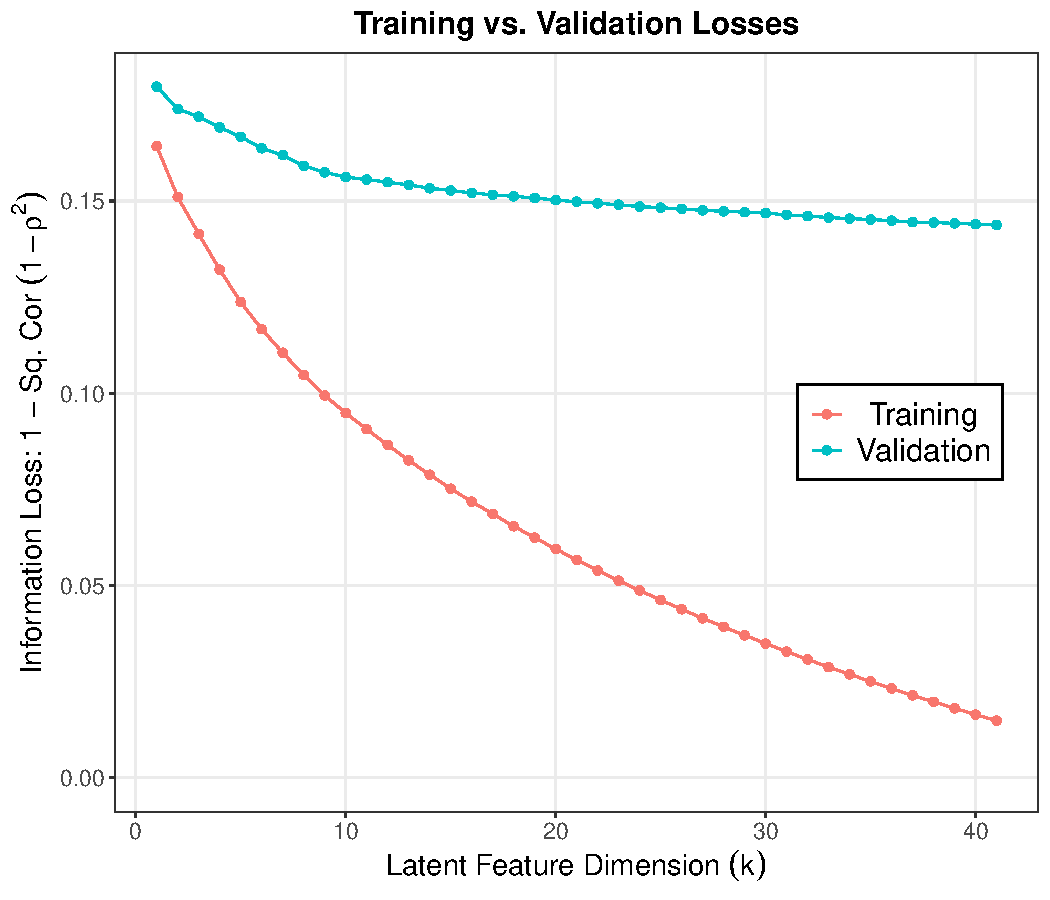
\includegraphics[width=0.5\linewidth]{figures/training-validation.pdf}
    \caption{Example of the average information loss from PCA of the Proteomic Gels data \parencite{morris_pinnacle_2008}, where the loss estimate is computed on the training sample (blue) vs. on a validation sample (red) (i.e., estimated via $5$-fold cross-validation).}
    \label{fig:training-validation}
\end{figure}


\begin{figure}
    \centering
    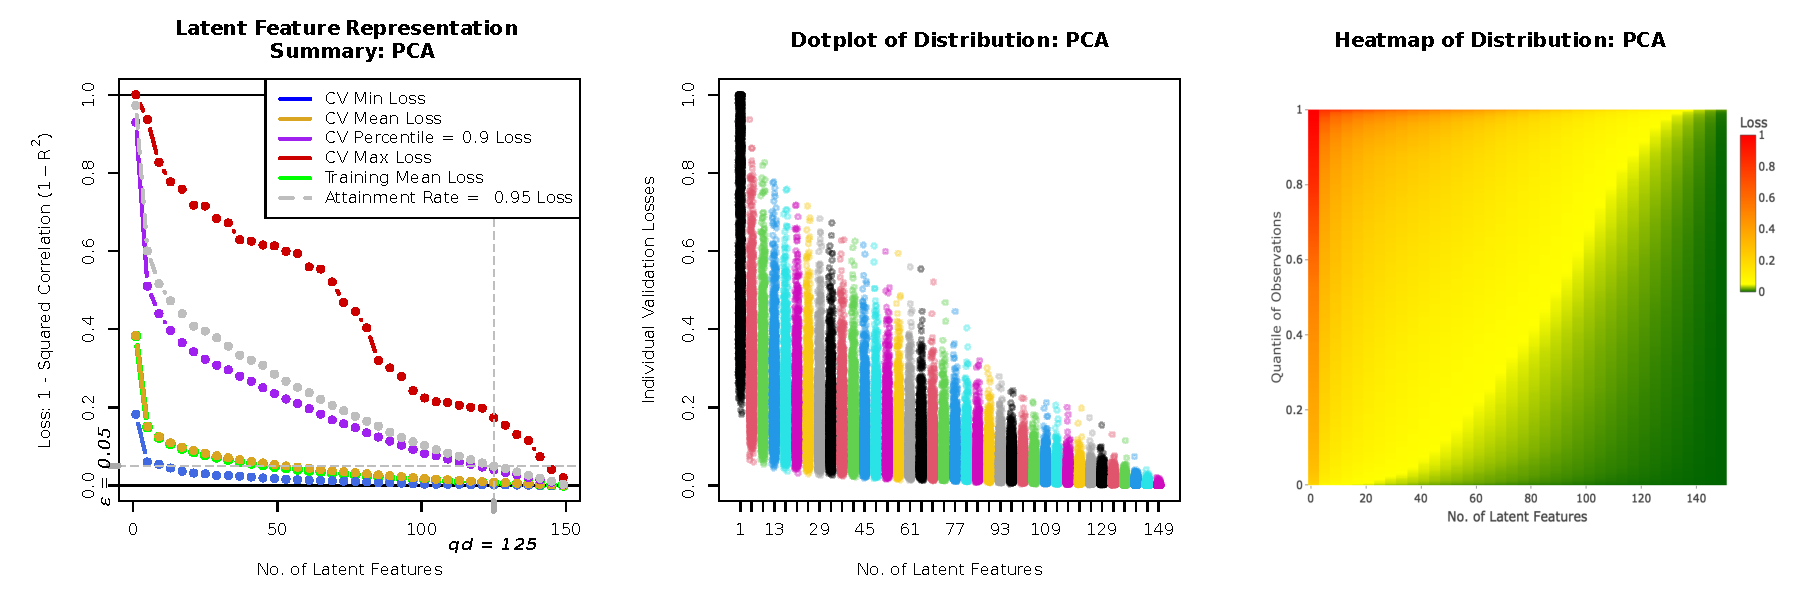
\includegraphics[width=1\linewidth]{figures/dist-summaries.pdf}
    \caption{Caption}
    \label{fig:enter-label}
\end{figure}

\begin{algorithm}
\caption{CoLLaRe Framework for Evaluating Latent Representations}
\begin{algorithmic}[1]

\State \textbf{Initialization} Start with a data matrix $\mathbf{X}$, a latent feature representation method (e.g., PCA, wavelets, or autoencoders) and a choice of loss function. Define the range of latent dimensions to evaluate and the number of folds for cross-validation. Set up a matrix to hold the cross-validated information losses for all observations (in rows) and latent dimensions (in columns).

\State \textbf{Generate cross-validation splits:} Randomly shuffle the dataset and then divide it into folds for cross-validation. Reuse these splits across all candidate latent feature dimensions for consistency and efficiency.

\State \textbf{For each candidate latent dimension $K$:}
\begin{enumerate}[a.]
    \item \textbf{For each cross-validation fold:}
    \begin{enumerate}[i.]
        \item \textbf{Train:Validation split:} 
        \begin{itemize}
            \item Split the data into training and validation sets for the current fold.
        \end{itemize}
        \item \textbf{Learn encoding and decoding transformations on training data:}
        \begin{itemize}
            \item Train a representation method (e.g., PCA, wavelets, or autoencoders) on the training data to learn the encoding and decoding transformations $f_K$ and $f^{-1}_K$.
        \end{itemize}
        \item \textbf{Reconstruct validation data:}
        \begin{itemize}
            \item Apply the learned transformations to encode and decode the validation dataset to give reconstructions $\widehat{X}_i (\mathbf{t})$ of $X_i (\mathbf{t})$.
        \end{itemize}
        \item \textbf{Compute information loss on validation data:}
        \begin{itemize}
            \item Measure the dissimilarity between the original and reconstructed validation data for each observation in the validation set using the loss function $g(\cdot, \cdot)$ and store these values.
        \end{itemize}
    \end{enumerate}
\end{enumerate}

\State \textbf{Identify the qualifying dimension:} For each latent dimension, compute the $\alpha$th quantile (e.g., 95th percentile) of the information loss across all observations as specified by the attainment rate $\alpha$. Select the smallest latent feature dimension where this quantile is below the specified tolerance level $\epsilon$.

\State \textbf{Re-train the model at the qualifying dimension:} If a qualifying dimension is identified, re-train the representation method using the full dataset at the qualifying dimension. Store the final trained model for downstream applications.

\State \textbf{Return results:} Return the full matrix of cross-validated information losses and, if applicable, the qualifying latent dimension and the final trained model at that dimension. If applying the algorithm to select among different methods, choose the method with the smallest qualifying dimension.

\end{algorithmic}
\end{algorithm}



\section{Software}\label{sec:software}

\begin{itemize}
    \item General structure of software.
    \item Demo line of code.
    \item GLaRe plot w/ labels.
    \item Default method implementations (PCA, DWT 1-D and 2-D, AE and architecture + packages) and how to define own function.
\end{itemize}
\section{Results of Case Studies}\label{sec:results}

This section presents the results of applying \texttt{GLaRe()} to our three motivating datasets --  the Glaucoma data (Section \ref{sec:glaucoma-reults}), the Proteomic Gels data (Section \ref{sec:gels-reults}) and the MNIST digits data (Section \ref{sec:mnist-reults}) -- to choose between our three built-in latent feature representation methods described in Section \ref{sec:learning-functions} -- Principal Components Analysis (PCA), the Discrete Wavelet Transform (DWT) and an autoencoder (AE).
For all three datasets, we use a tolerance level of $\epsilon = 0.05$ and cut-off criterion of $\alpha=0.95$ with hyperparatmeters and settings for the methods set at their defaults outlined in Section \ref{sec:learning-functions} unless otherwise specified.
Finally, in Section \ref{sec:sample-size-experiment}, we perform an experiment where we artificially decimate the sample size of the Glaucoma dataset to demonstrate the dependence of PCA and the DWT on different sample sizes.
Additional results of the case studies are presented in Appendix \ref{sec:additional-results}.

\subsection{Glaucoma Data}\label{sec:glaucoma-reults}

Figure \ref{fig:eye-results} displays the summary plot from the application of \texttt{GLaRe()} to the Glaucoma data.
PCA is the most suitable latent feature representation method for this dataset because it achieves the qualifying criterion at $K=51$, whereas DWT and AE do not achieve the qualifying criterion for $K \leq 261$.
A grid of equally-spaced values from $1$ to $261$ in increments of $10$ was used for the latent feature dimensions. 
Although it was possible to use larger latent feature dimensions for the DWT and AE, the qualifying criterion was achieved for PCA at $K=51$ so it was deemed unnecessary.
The computation times for PCA, DWT and AE were $1.2$, $0.7$ and $69.4$ minutes, respectively.


\begin{figure}
    \centering
    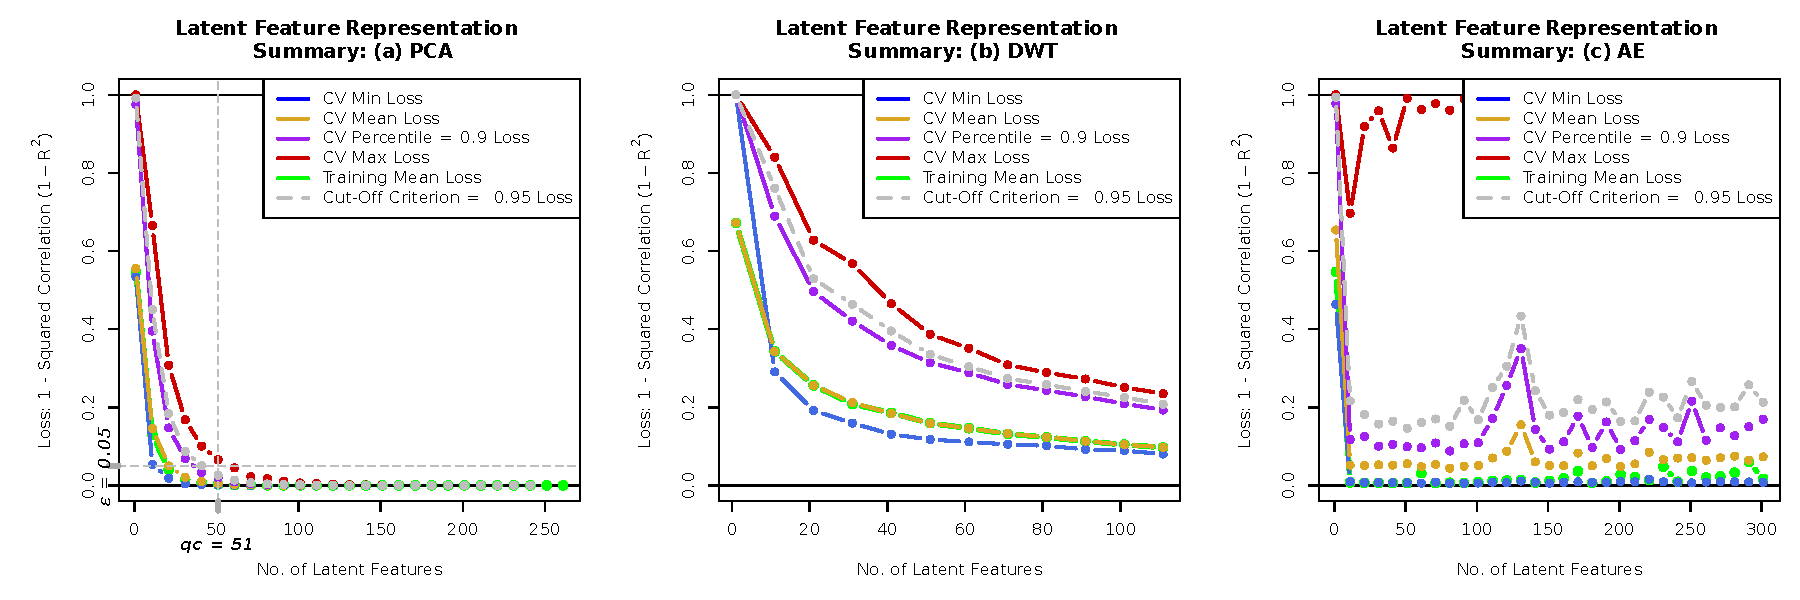
\includegraphics[width=1\textwidth]{figures/eye-results.pdf}
    \caption{Summary \texttt{GLaRe()} plot for the Glaucoma data. A grid of equally-spaced values from $1$ to $261$ in increments of $10$ was used for the latent feature dimensions.}
    \label{fig:eye-results}
\end{figure}

\subsection{Proteomic Gels Data}\label{sec:gels-reults}

\begin{figure}
    \centering
    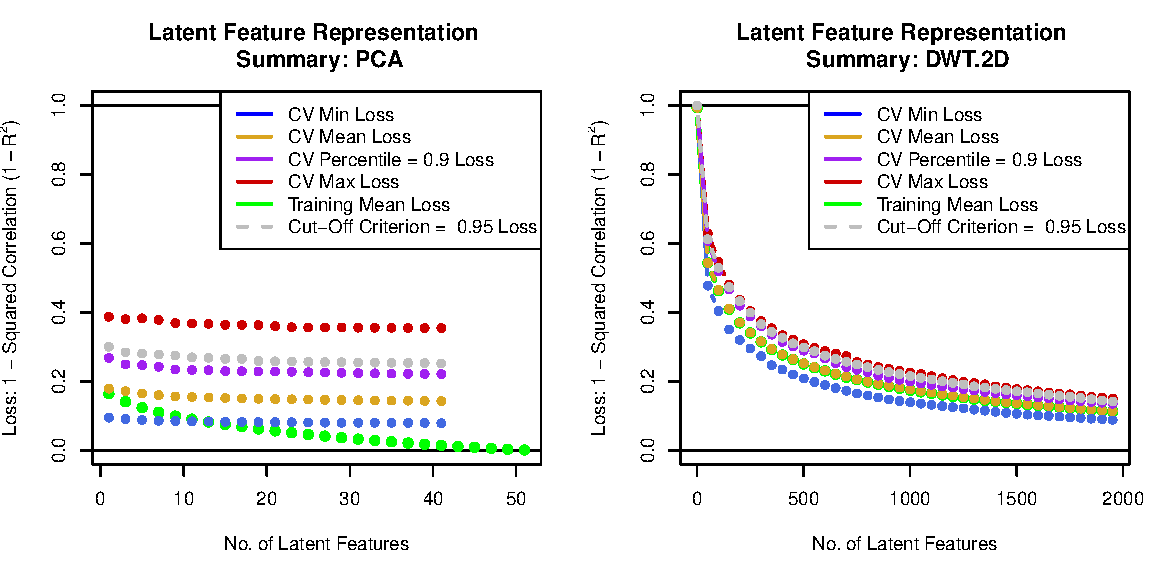
\includegraphics[width=1\linewidth]{figures/initial-gels.pdf}
    \caption{Preliminary results for the gels data.}
    \label{fig:enter-label}
\end{figure}


\subsection{MNIST Digits Data}\label{sec:mnist-reults}

Figure \ref{fig:mnist-results} displays the summary plot from the application of \texttt{GLaRe()} to the MNIST data.
PCA is the most suitable latent feature representation method for this dataset because it achieves the qualifying criterion at $K=201$, whereas DWT achieved it at $K=321$ and the AE did not achieve the qualifying criterion for $K \leq 381$.
A grid of equally-spaced values from $1$ to $381$ in increments of $20$ was used for the latent feature dimensions. 
The computation times for PCA, DWT and AE were $X_1$, $X_2$ and $X_3$ minutes, respectively.

\begin{figure}
    \centering
    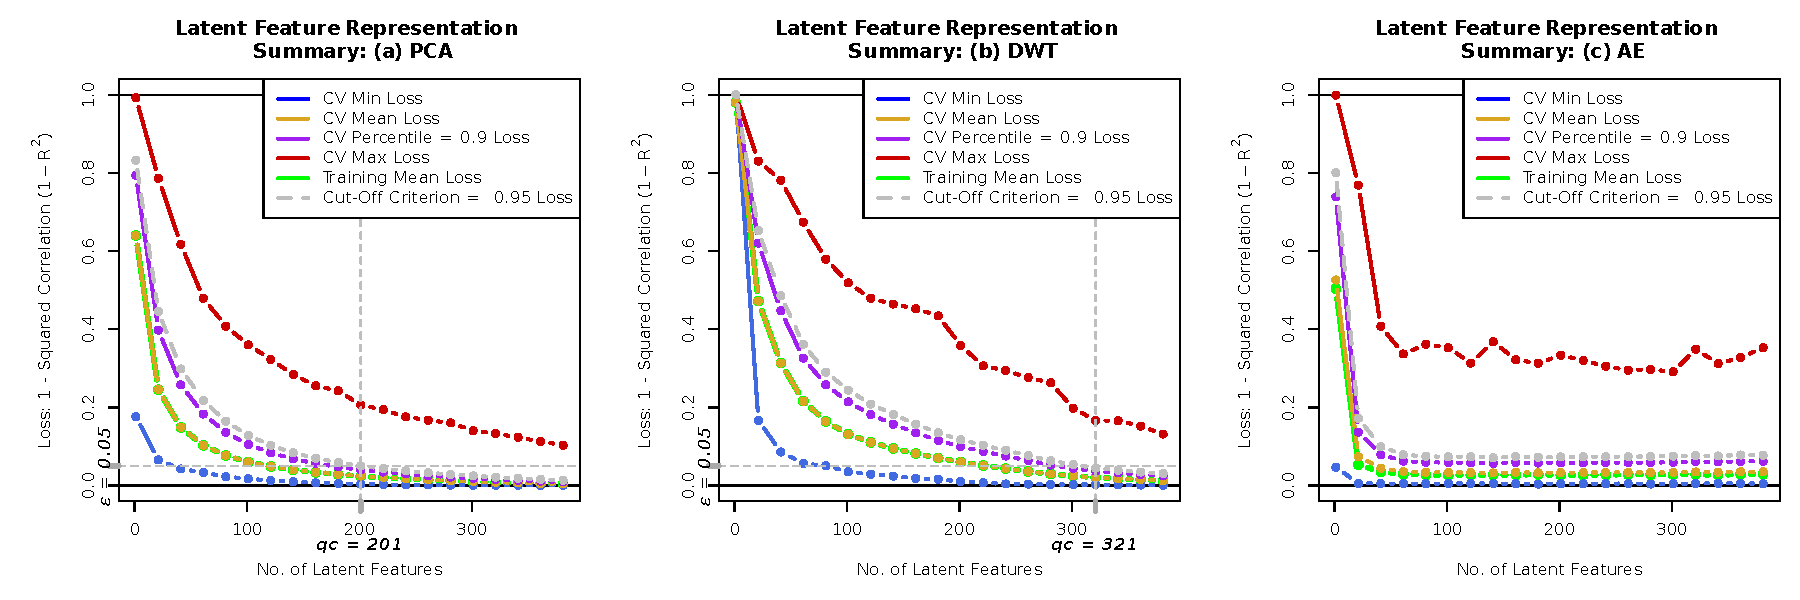
\includegraphics[width=1\textwidth]{figures/mnist-results.pdf}
    \caption{Summary \texttt{GLaRe()} plot for the MNIST data. A grid of equally-spaced values from $1$ to $381$ in increments of $20$ was used for the latent feature dimensions.}
    \label{fig:mnist-results}
\end{figure}

\subsection{Sample Size Experiment}\label{sec:sample-size-experiment}


\begin{figure}
    \centering
    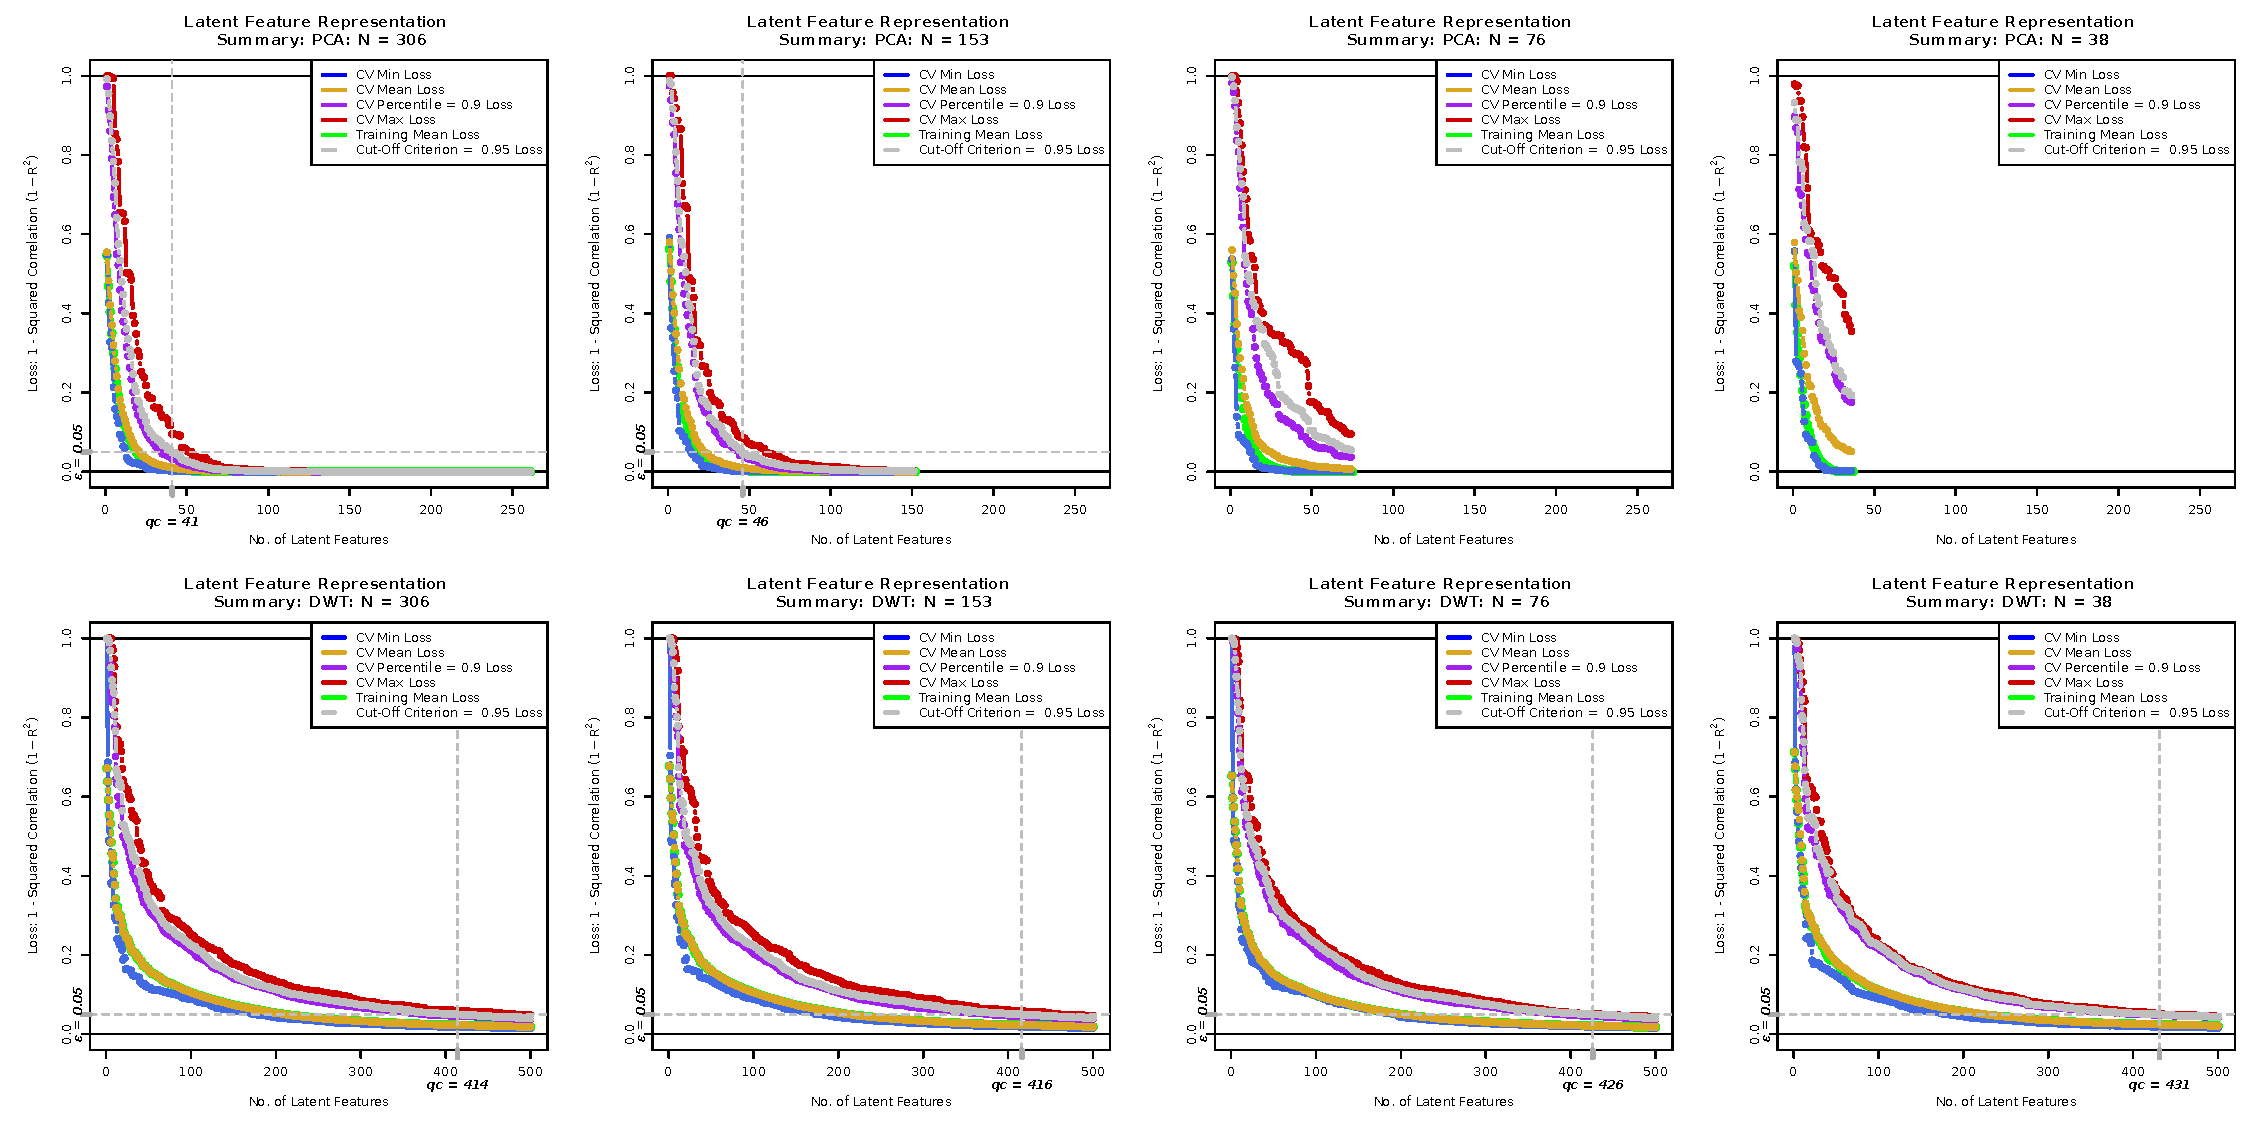
\includegraphics[width=1\linewidth]{figures/eye-sample-size-results-results-01.pdf}
    \caption{Caption}
    \label{fig:eye-sample-size-results-results-01}
\end{figure}



\section{Discussion}\label{sec:discussion}

We have introduced CoLLaRe, an evaluation framework for assessing and comparing latent feature representation methods with a focus on compactness and (near-)losslessness.
A distinguishing feature of CoLLaRe is its focus on the full distribution of generalization errors rather than aggregated metrics such as average or total information loss.
Our framework uses cross-validation to estimate the full distribution of generalization errors and proposes to choose a representation such that a tolerance level of generalization error is met for generalized quantiles of this distribution (e.g., worst case or $95$th percentile) while ensuring that the representation is as compact as possible.
Thus, CoLLaRe enables the selection of a compact, near-lossless latent feature representations that ensures statistical modeling in the latent space can accurately reflect the underlying mechanisms of the true data-generating process.


% Unlike traditional approaches that rely on single summary metrics that are aggregated over all observations, GLaRe provides a more nuanced evaluation, capturing variability across individual observations.
% To characterize this distribution, we introduced key concepts such as the tolerance level, cut-off criterion, and qualifying dimension, which enable tailored assessments of latent feature representation methods.
% We have provided an accompanying software package GLaRe which implements the framework and provides interpretable graphical summaries.


One of CoLLaRe's strengths is that it facilitates comparisons between methods, allowing comparisons between traditional tools such as PCA and modern approaches such as autoencoders. 
Through case studies on three datasets—Glaucoma, Proteomic Gels, and MNIST, we have demonstrated how CoLLaRe can guide the selection of the most suitable latent feature representation based on dataset characteristics.
The results from these case studies reinforce the importance of such context-specific evaluation, as the preferred representation method varied across datasets. 
For instance, the MNIST dataset, with its large sample size relative to feature dimension, benefited from the flexibility of the non-linear AE representation. 
In contrast, for the Proteomic Gels dataset, which is characterized by a small sample size relative to its high-dimensional features, the fixed DWT representation was preferred to the more flexible PCA and AE representations.
We performed an experiment by manually decreasing the sample size of the Glaucoma dataset and comparing the PCA and DWT representations which further highlighted the trade-off between flexible methods and sample size.
These case studies emphasize the role of dataset characteristics, such as sample size, dimensionality and variance structure, in determining the most appropriate latent feature representation. 
CoLLaRe is a valuable framework to compare methods under a consistent set of criteria in such contexts.

We have also described and documented our accompanying \proglang{R} package, GLaRe, which implements the CoLLaRe framework and provides intuitive graphical summaries for the user.
GLaRe provides a flexible implementation of the framework where the user can specify the criteria (e.g., tolerance level, attainment rate).
It provides built-in implementations of three latent feature representation methods -- PCA, DWT and autoencoder -- but it also allows the user to easily specify specify a latent feature representation method of their own..
It is publicly available and can be employed by practitioners in any analysis that relies on latent feature representation methods.


% GLaRe places a unique focus on estimating the full distribution of generalization error for a given dataset, which is more sensitive and informative than summary or total measures.
% We have coined new terminology, e.g., ``tolerance level", ``cut-off criterion", ``qualifying dimension" and ``qualifying criterion", to characterize this distribution and use it to assess latent feature representation methods.
% Our software produces a summary plot as well as several other visualizations to summarize and characterize this distribution.

% A key feature of GLaRe is that it is not tied to any latent feature representation method and can be used to compare among several methods, as demonstrated through our case studies.
% The results of these case studies emphasize the utility of GLaRe, as each of the motivating datasets favored a different latent feature representation method.
% They also re-enforce that sample size plays (alongside data structure) an important role when choosing a latent feature representation method.
% For the MNIST dataset, the sample size ($N=60000$) is large relative to the feature dimension ($T=784$) so it was possible to estimate a flexible non-linear transformation of the data using the AE that provided an optimal representation of the data.
% On the other hand, the Proteomic Gels data has a small sample size ($N=53$) relative to the feature dimension ($T=556206$) so the fixed DWT representation was preferred to the more flexible PCA and AE representations.
% We performed an experiment by manually decreasing the sample size of the Glaucoma dataset and comparing the PCA and DWT representations which further highlighted the trade-off between flexible methods and sample size.
% These case studies underscore the critical role of dataset characteristics, such as sample size and dimensionality, in determining the most appropriate latent feature representation. 
% CoLLaRe's flexibility in comparing methods under consistent criteria is particularly valuable in such contexts.


Some limitations and future directions of this work are as follows.
Our framework focuses on compactness and near-losslessness, which are two of the most important properties of a latent feature representation.
However, other properties might also need to be considered when selecting among representations, e.g., distribution of features in the latent space, interpretability of the latent features, computational time, and effort.
The current framework should also be extended to handle dependent (e.g., multilevel, longitudinal, temporal/ spatial) data by including structured variants of cross-validation for dependent datasets
\parencite{bergmeir_note_2018, hornung_evaluating_2023, roberts_cross-validation_2017}.
In our case studies, we used standard versions of PCA, DWT and AE to facilitate general and straightforward comparisons but future work could consider specialized implementations (e.g., smoothed functional PCA or convolutional autoencoders). 
Finally, from a software development perspective, the addition of a Graphical User Interface (GUI) using \proglang{Shiny} \parencite{chang_shiny_2021}, parallelization of the cross-validation algorithm and the addition of new wrapper functions is of interest.

% {\color{purple}FIX THIS!}

% Firstly, we focused on providing standard, rather than specialized, implementations of PCA and the AE.
% While it is possible to use the \texttt{learn = "user"} setting to specify user-defined transformations, e.g., smoothed functional PCA for curve data or convolutional AEs for image data, a future direction is to build these methods in along the standard PCA, DWT and AE options.
% Likewise, we favored the squared correlation loss due to its tractability and inherent links to conventional loss quantities in classical PCA (Appendix \ref{sec:squared-correlation}), but our software is structured such that future iterations can use alternative other loss functions \parencite[e.g., concordance index, see][]{yang_quantile_2020} that are specified or provided by the user.
% It would also be useful to include structured variants of cross-validation for dependent datasets (e.g., hierarchical, longitudinal or spatial/ temporal dependence structures) \parencite{bergmeir_note_2018, hornung_evaluating_2023, roberts_cross-validation_2017}.
% From a software development perspective, the addition of a Graphical User Interface (GUI) using \proglang{Shiny} \parencite{chang_shiny_2021}, parallelization of the cross-validation algorithm and the addition of new wrapper functions is of interest.

%----------------------------%
\section*{Supporting Information}

Appendices \ref{sec:additional-data}-\ref{sec:additional-results} contain additional details of the analysis.
\proglang{R} code scripts and data to reproduce the analysis are available at \proglang{GitHub}\footnote{ \url{https://github.com/edwardgunning/MANUSCRIPT-CLaRe}.}.

\section*{Acknowledgements}
We are grateful to Martin Das (Sr. Software and Technical Specialist) for his computational assistance.
An early draft of this work first appeared as part of Dr. Emma Zohner's Ph.D. dissertation (\citeyear{zohner_feature_2021}, Chapter 2).
This work was partially supported by the following grants: CA-244845 and CA-178744.
\clearpage

\appendix
\section{Wavelet Thresholding Algorithm}

\item \pkg{wavselim} \proglang{R} package.

\begin{steps}
  \item \underline{Pad the Data to Ensure Dyadic Length}:
  \item Second thing to do
  \item Third thing to do
\end{steps}

\begin{enumerate}
    \item 
\end{enumerate} 
\clearpage
\printbibliography
\end{document}
